\documentclass[12pt,letterpaper,english]{article}
\usepackage{times}
\usepackage[T1]{fontenc}
\IfFileExists{url.sty}{\usepackage{url}}
                      {\newcommand{\url}{\texttt}}

\usepackage{babel}
\usepackage{Rd}

\usepackage{Sweave}

\begin{document}
\Sconcordance{concordance:LoSharpe.tex:LoSharpe.Rnw:%
1 27 1 1 4 1 5 21 1 1 2 1 0 1 2 5 0 1 2 1 1 1 2 1 0 1 1 1 2 1 0 1 2 5 0 %
1 2 2 1}


\title{ Lo Sharpe Ratio }
\author{R Project for Statistical Computing}
% \keywords{Lo Sharpe Ratio,GLM Smooth Index,GLM Return Table}

\makeatletter
\makeatother
\maketitle

\begin{abstract}

    This vignette gives an overview of the Lo Sharpe Ratio which have addressed the issue of IID in the financial time series data.
\end{abstract}



\section{Background}
The building blocks of the \textbf{Sharpe Ratio} : expected returns and volatilities  are unknown quantities that must be estimated statistically and are,
therefore, subject to \emph{estimation error} . This raises the natural question: How
\emph{accurately} are Sharpe ratios measured? To address this question, Andrew Lo derives explicit expressions for the statistical distribution of the Sharpe ratio using
standard asymptotic theory. 


\section{Lo Sharpe Ratio}
 Given a predefined benchmark Sharpe ratio , the observed Sharpe ratio       can be expressed in terms of autocorrelated coefficients as
 
 \deqn{ \hat{SR} (q) - SR(q)= Normal Distribution(0,V_{GMM}(q)) }
 
The estimator for the Sharpe ratio then follows directly:
\deqn{  \hat{SR} (q) =  \hat{ \eta } (q)  * Sharpe Ratio}
\deqn{  \hat{ \eta } (q)= q/\sqrt{q +  \sum_k^n  \rho  } }
\section{Example}

In an illustrative
empirical example of mutual funds and hedge funds, we find results, similar reported in paper, that the annual Sharpe ratio for a hedge fund can be overstated by as much as \textbf{65} \% because of the presence of \textbf{serial correlation} , and once
this serial correlation is properly taken into account, the rankings of hedge
funds based on \emph{Sharpe ratios} can change dramatically.

\begin{Schunk}
\begin{Sinput}
> data(edhec)
> charts.PerformanceSummary(edhec[,2:4],
+ colorset = rich6equal, lwd = 2, ylog = TRUE)
\end{Sinput}
\end{Schunk}
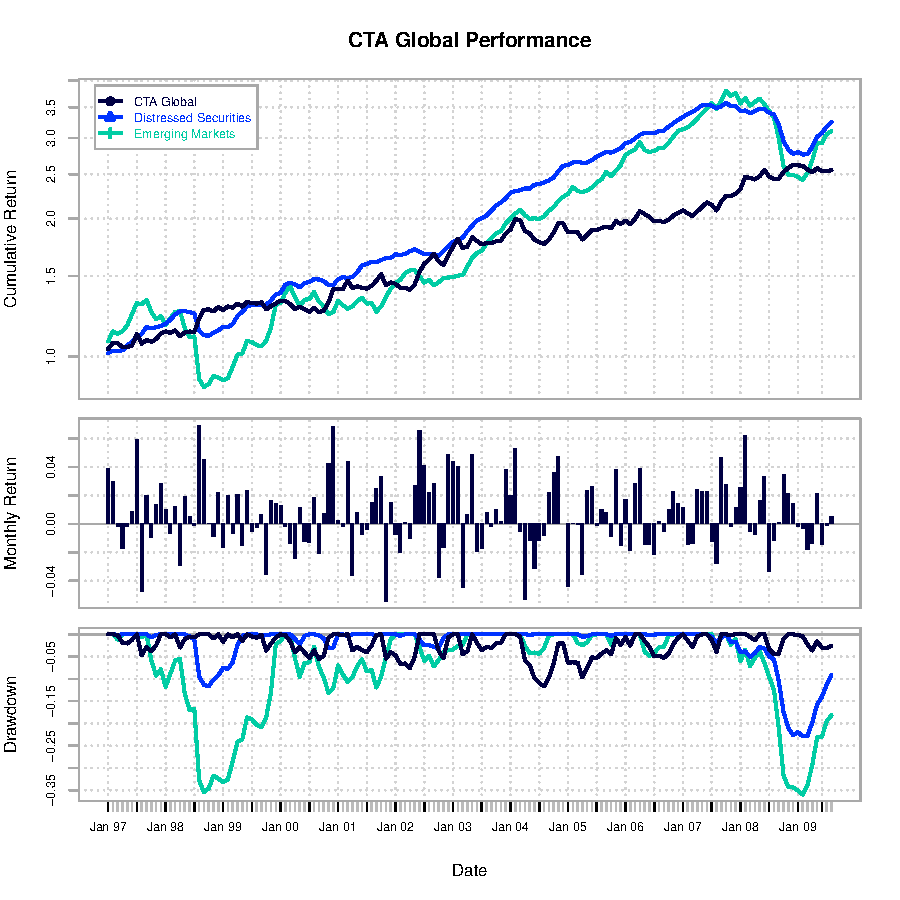
\includegraphics{LoSharpe-003}

We can observe that the fund "\textbf{Emerging Markets}", which has the largest drawdown and serial autocorrelation, has it's Andrew Lo Sharpe ratio , \emph{decrease} most significantly as comapared to other funds.
\begin{Schunk}
\begin{Sinput}
> Lo.Sharpe = LoSharpe(edhec[,2:4])
> Theoretical.Sharpe= SharpeRatio.annualized(edhec[,2:4])
> barplot(rbind(Theoretical.Sharpe,Lo.Sharpe), main="Theoretical and Andrew Lo Sharpe Ratio Observed",
+          xlab="Fund Type",ylab="Value", col=c("darkblue","red"), beside=TRUE)
>    legend("topright", c("1","2"), cex=0.6, 
+                    bty="2", fill=c("darkblue","red"));
\end{Sinput}
\end{Schunk}
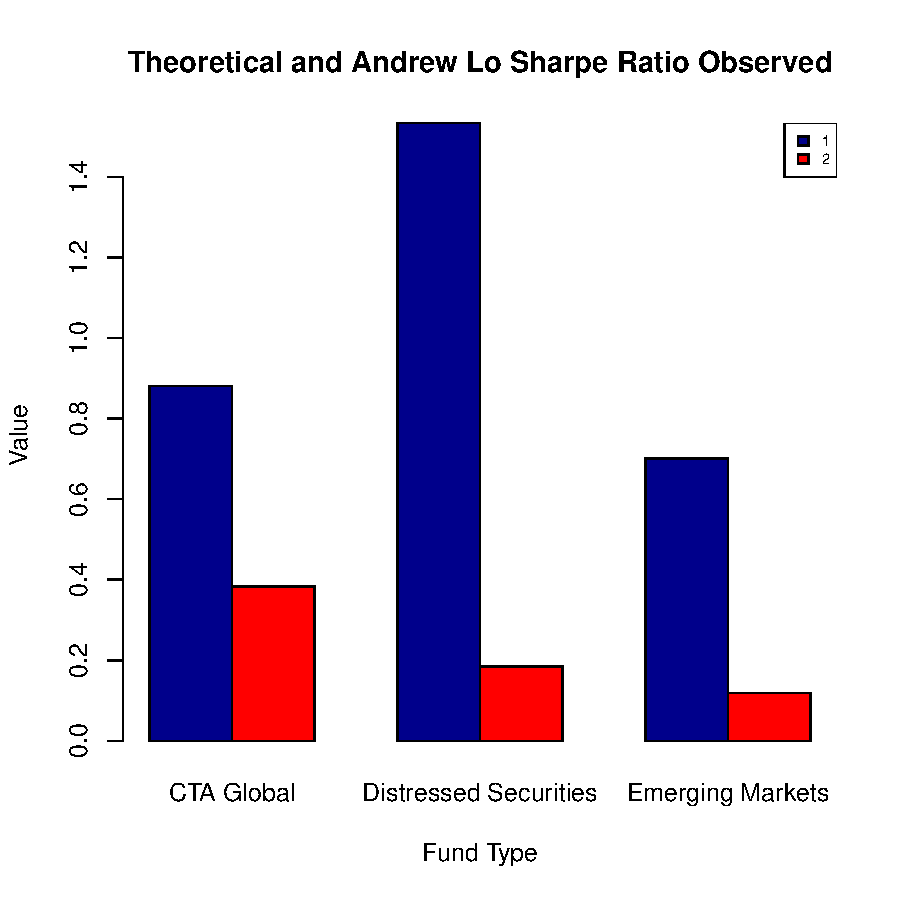
\includegraphics{LoSharpe-004}


\end{document}
